\documentclass[11pt, oneside]{article}   % use "amsart" instead of "article" for AMSLaTeX format
\usepackage{geometry}
\usepackage{graphicx}                    % used for pdf figures
\usepackage[fleqn]{amsmath}

\geometry{letterpaper}                   % ... or a4paper or a5paper or ... 

\title{Inverse Kinematics of the Robotic Manipulator}
\author{Patrick Scheffe, Nikolas Alberti}

\begin{document}
\maketitle

\section{Simplified Kinematic Model}\label{section1}

A simplified sketch of the robotic manipulator can be seen in Figure \ref{fig:model}.
As a first approximation it is useful to determine the angles $\theta_1$ to $\theta_4$ from the given position of the joint at which the two arms coincide (x,y). The key for solving this inverse kinematics problem is to divide it into smaller subproblems that each can be solved individually. For that purpose, the line segments $a$, $b$ and $c$ are introduced.
\begin{figure}[!h]
\label{fig:model}
  \centering
      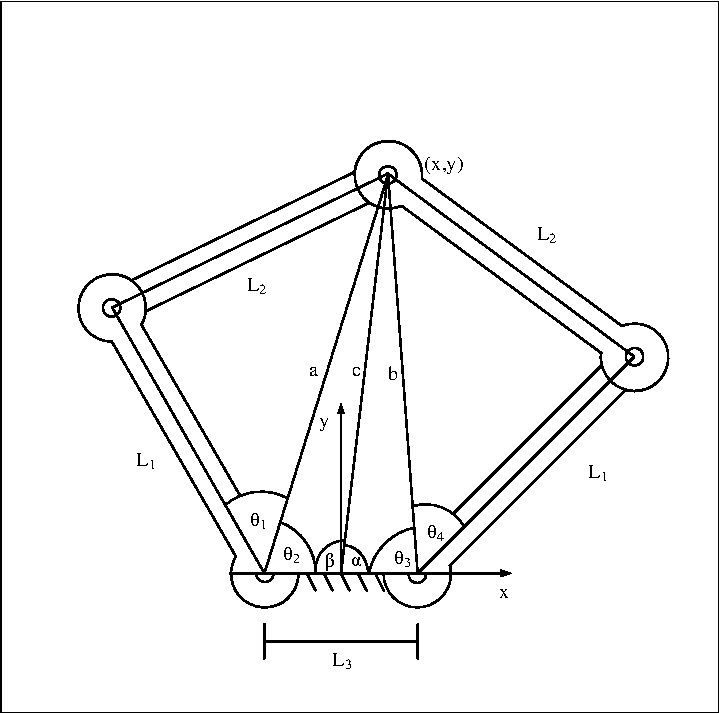
\includegraphics[scale=1]{LinkDiagramSimple_try.pdf}
  \caption{Simplified Version of the Manipulator}
\end{figure}

From the initial information, following values can be directly computed:
\begin{equation}
\alpha = arctan \left( \frac{y}{x} \right)
\end{equation}
\begin{equation}
\beta = \pi - \alpha
\end{equation}
\begin{equation}
c = \sqrt{x^2 + y^2}
\end{equation}
\begin{equation}
a = \sqrt{\left(x+ \frac{L_3}{2}\right)^2 + y^2}
\end{equation}
\begin{equation}
b = \sqrt{\left(x- \frac{L_3}{2}\right)^2 + y^2}
\end{equation}


Now, you can solve for $\theta_2$ and $\theta_3$ by either using sine rule or cosine rule. However, the sine rule can be ambiguous in certain setups, which makes case differentiation necessary. Although mathematically steady, in our implementation the domain crossing from one solution to the other resulted in discontinuities of the movement. Therefore, the cosine rule solution is preferred:
\begin{equation}
\theta_2 = arccos\left(  \frac{a^2 + (\frac{L_3}{2})^2 - c^2}{aL_3} \right)
\label{eqn:theta2}
\end{equation}
\begin{equation}
\theta_3 = arccos\left(  \frac{b^2 + (\frac{L_3}{2})^2 - c^2}{bL_3} \right)
\label{eqn:theta3}
\end{equation}


Using cosine rule we can also solve for $\theta_1$ and $\theta_4$:
\begin{equation}
\theta_1 = arccos\left(  \frac{a^2 + {L_1}^2 - {L_2}^2}{2aL_1} \right)
\label{eqn:theta1}
\end{equation}

\begin{equation}
\theta_4 = arccos\left(  \frac{b^2 + {L_1}^2 - {L_2}^2}{2bL_1} \right)
\label{eqn:theta4}
\end{equation}

\section{Complete Kinematic Model}
The simplified version of the kinematic model is good for quickly creating a working implementation. However, any movements executed by the manipulator will suffer from distortion. The pen is not mounted \emph{exactly} at the joint's position but in a small distance. Hence, a precise solution is necessary. For that purpose, new definitions must be made (Figure \ref{fig:model2}).
\begin{figure}[!h]
	\label{fig:model2}
	\centering
	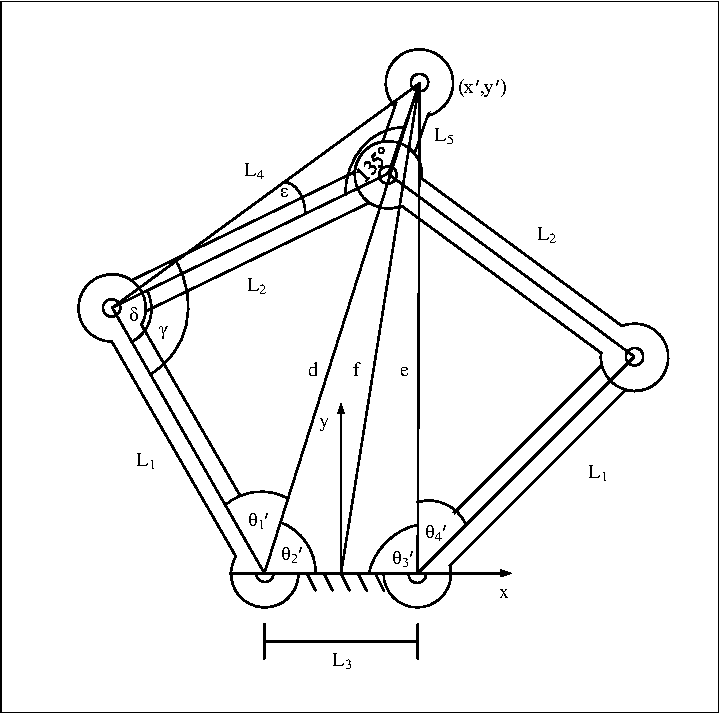
\includegraphics[scale=1]{LinkDiagramComplicated_try.pdf}
	\caption{Simplified Version of the Manipulator}
\end{figure}

$L_4$ and $\epsilon$ are fixed measures and not influenced by the position of the manipulator:
\begin{equation}
L_4 = \sqrt{{L_2}^2 + {L_5}^2 - 2L_5L_2cos\left(\frac{3\pi}{4}\right)}
\label{eqn:L4}
\end{equation}
\begin{equation}
\epsilon = arccos\left(  \frac{{L_4}^2 + {L_2}^2 - {L_5}^2}{2L_4L_2} \right)
\label{eqn:tepsilon}
\end{equation}

$d$, $e$ and $f$ can be yielded by the Pythagorean theorem:
\begin{equation}
f = \sqrt{{x'}^2 + {y'}^2}
\label{eqn:f}
\end{equation}
\begin{equation}
d = \sqrt{\left(x'+ \frac{L_3}{2}\right)^2 + {y'}^2}
\end{equation}
\begin{equation}
e = \sqrt{\left(x'- \frac{L_3}{2}\right)^2 + {y'}^2}
\end{equation}
Now, $\theta_2'$, $\theta_3'$ and $\delta$ can be computed using cosine rule:
\begin{equation}
\theta_2' = arccos\left(  \frac{d^2 + (\frac{L_3}{2})^2 - f^2}{dL_3} \right)
\label{eqn:theta2prime}
\end{equation}
\begin{equation}
\theta_3' = arccos\left(  \frac{e^2 + (\frac{L_3}{2})^2 - f^2}{eL_3} \right)
\label{eqn:theta3prime}
\end{equation}
\begin{equation}
\delta = arccos\left(  \frac{{L_4}^2 + {L_1}^2 - d^2}{2L_4L_1} \right)
\label{eqn:delta}
\end{equation}
$\delta$ is the sum of $\epsilon$ and $\gamma$.
\begin{equation}
\gamma = \delta - \epsilon
\end{equation}
That allows us to calculate some quantities of the simple kinematics model:
\begin{equation}
a = \sqrt{{L_1}^2 + {L_1}^2 - 2L_1L_2cos\left(\gamma\right)}
\end{equation}
\begin{equation}
\theta_1 = arccos\left(  \frac{a^2 + {L_1}^2 - {L_2}^2}{2aL_1} \right)
\end{equation}
\begin{equation}
\theta_2 = \theta_1' + \theta_2' - \theta_1
\end{equation}
Finally, we are able to find the position of the joint at which the two arms coincide:
\begin{equation}
	y = a \sin(\theta_2)
\end{equation}
\begin{equation}
	x = a\cos(\theta_2) - \frac{L_3}{2}
\end{equation}
Now, the methods from section \ref{section1} can be used to solve for $\theta_3$ and $\theta_4$.


\end{document}  

















